\documentclass{article}

\usepackage[utf8]{inputenc}

\usepackage[backend=biber,style=authoryear,]{biblatex}
%%%%%%%%%%%%%%%%%%%%%%%%%%%%%%%%%%%%%%%%%
% Arsclassica Article
% Structure Specification File
%
% This file has been downloaded from:
% http://www.LaTeXTemplates.com
%
% Original author:
% Lorenzo Pantieri (http://www.lorenzopantieri.net) with extensive modifications by:
% Vel (vel@latextemplates.com)
%
% License:
% CC BY-NC-SA 3.0 (http://creativecommons.org/licenses/by-nc-sa/3.0/)
%
%%%%%%%%%%%%%%%%%%%%%%%%%%%%%%%%%%%%%%%%%

%----------------------------------------------------------------------------------------
%	REQUIRED PACKAGES
%----------------------------------------------------------------------------------------

\usepackage[
nochapters, % Turn off chapters since this is an article        
beramono, % Use the Bera Mono font for monospaced text (\texttt)
eulermath,% Use the Euler font for mathematics
pdfspacing, % Makes use of pdftex’ letter spacing capabilities via the microtype package
dottedtoc % Dotted lines leading to the page numbers in the table of contents
]{classicthesis} % The layout is based on the Classic Thesis style

\usepackage{arsclassica} % Modifies the Classic Thesis package
%\usepackage{fancyhdr}
\usepackage[T1]{fontenc} % Use 8-bit encoding that has 256 glyphs

\usepackage[utf8]{inputenc} % Required for including letters with accents
%\pagenumbering{arabic}
\usepackage[margin=1in,footskip=.25in]{geometry}
\usepackage{wrapfig}
\usepackage{graphicx} % Required for including images
\graphicspath{{Figures/}} % Set the default folder for images

\usepackage{enumitem} % Required for manipulating the whitespace between and within lists

\usepackage{lipsum} % Used for inserting dummy 'Lorem ipsum' text into the template

\usepackage{subfig} % Required for creating figures with multiple parts (subfigures)

\usepackage{amsmath,amssymb,amsthm} % For including math equations, theorems, symbols, etc

\usepackage{multirow} % for including eqs in multirows

\usepackage{varioref} % More descriptive referencing

\usepackage{floatflt,epsfig} % for including figure in the text

\usepackage{wrapfig}
%----------------------------------------------------------------------------------------
%	THEOREM STYLES
%---------------------------------------------------------------------------------------

\theoremstyle{definition} % Define theorem styles here based on the definition style (used for definitions and examples)
\newtheorem{definition}{Definition}

\theoremstyle{plain} % Define theorem styles here based on the plain style (used for theorems, lemmas, propositions)
\newtheorem{theorem}{Theorem}

\theoremstyle{remark} % Define theorem styles here based on the remark style (used for remarks and notes)

%----------------------------------------------------------------------------------------
%	HYPERLINKS
%---------------------------------------------------------------------------------------

\hypersetup{
%draft, % Uncomment to remove all links (useful for printing in black and white)
colorlinks=true, breaklinks=true, bookmarks=true,bookmarksnumbered,
urlcolor=webbrown, linkcolor=RoyalBlue, citecolor=webgreen, % Link colors
pdftitle={}, % PDF title
pdfauthor={\textcopyright}, % PDF Author
pdfsubject={}, % PDF Subject
pdfkeywords={}, % PDF Keywords
pdfcreator={pdfLaTeX}, % PDF Creator
pdfproducer={LaTeX with hyperref and ClassicThesis} % PDF producer
}

 
\addbibresource{sample.bib}

%\bibliography{sample}
\title{PhD Report - Faculty of Biological Science -\\University of Heidelberg Ruperto Carola}
\author{Carla Filosa}
\date{---------------------------------------------------}

\begin{document}

\maketitle
\setcounter{tocdepth}{2} % Set the depth of the table of contents to show sections and subsections only

\tableofcontents % Print the table of contents

%\listoffigures % Print the list of figures

%\listoftables % Print the list of tables
\section{Introduction}
% CIAO CARLA
Ensemble analysis, namely the plethora of methods developed by scientist with the aim to individuate specific patterns in a system, has a central role in neuroscience. The individuation of activation neuron patterns can give us insights about the neural network working, since they can be generated either by anatomically or functionally connected groups of neurons.
In this report I show the application of an ensemble-detection-method in spike counts data, on spike data recorded from mice or rats brain when they perform different type of tasks. 
Neuronal systems are characterized by the presence of different time scales having a role in the neural response during a specific task. This beauty is unfortunately not easy to detect: the major part of ensemble methods in fact are able to find activation patterns only at one of the several time scales in which the patterns are activated, with a consequent information loss.
In the list of factors that plague data analysis in neuroscience a big role is played by the non-stationarity artefacts present in experimental data.
For these reasons a new method, able to remove many non-stationary artefacts and to individuate neuron patterns at different time scales, is chosen in my doctorate project analysis.
\section{What is a cell assembly?}
The fundamental concept of cell assembly was introduced by Hebb in the 1949. After more than six decades this idea continue to play a key role in our understanding of how neural physiology may link to cognitive function.
In few words a cell assembly refers to a group of neurons which, by functionally organizing into a temporally coherent set, come to represent mental or perceptual entities, thereby forming the basis  of neural coding and computation (\cite{Hebb}). However this definition is not precise and under the term cell assembly scientists have for long years included anything from precise zero-phase-lag spike synchronization in a defined subset of neurons to temporally coherent changes in average firing rates or larger time scale. That means that for different time scales, different type of assemblies exist associated to the different neurons patterns.
Recentely Russo and Durstewitz introduced a method able to detect different typologies of assemblies in multi-cell electrophysiological recording being able to distinguish different processes at different time scales, and as well to remove many non-stationary artefacts that plague data analysis in neuroscience (\cite{RussoDurstewitz}).
The detected pattern occur with a frequency that is higher the chance level and can be generated either by anatomically or functionally connected groups of neurons.


In figure (\ref{fig: AsEx}) we see an example of different possible detectable patterns . 
\begin{figure}[!ht]
  \begin{center}
    \includegraphics[width=1\textwidth]{AsEx1}
  \end{center}
\caption{\footnotesize{Detection of assemblies defined by different degrees of temporal precision, scale, and internal structure. Different assembly types in simulated non-stationary spike train: I - highly precise lag-0 synchronization; II- precise sequential pattern; III - precise-spike-time patterns without clear sequential structure; IV - rate pattern with temporal structure; V - simultaneous rate increase. Figure reproduced and modified from (\cite{RussoDurstewitz})}}
\label{fig: AsEx}
\end{figure}


\section{The ensemble detection method}
We won't go in the details of the method, that are explained in (\cite{RussoDurstewitz}), we rather show a schematic idea trough simple but fundamental steps. We intend to show the strength of the method instead with applying it on really data, and exploring also the different possible applications, as well investigating the kind of information that the assemblies carry on.
The method is based on counting spike occurrences of two units A,B. The idea proposed is using  multiple bin widths $\Delta$ and time lags $l$ to capture different neural patterns at different time scales. With the word pattern we intend objects that are not independent each other, or better, we define with the word pattern objects generated by anatomically or functionally connected groups of neurons. Keeping in mind this definition, the core of algorithm is easy to understand if we have only one basic mathematical notion:
\begin{itemize}
    \item For two independent data set $A, B$ the joint distribution of spike occurrences $p(A,B)$ at specific lag $l$ can be factor int single unit marginal distribution $p(A,B)=p(A)p(B)$
\end{itemize}
For spiking data we have a time series $\{c_t\}$ of spike counts of length $T$, we should chose a bin width $\Delta$ small enough to guarantee: $c_t \in \{0,1\}$, $\#_A$ and $\#_B$ is the total number of spikes of $A$ and $B$ respectively. The null Hypothesis ($H_0$) of independence asserts the following:
\begin{itemize}
    \item The joint spike count $\#_{A,B}$ at the time lag $l$ follows a hypergeometric distribution with mean: $\mu_{A,B} = \frac{\#_A \#_B}{T-l}$ and variance $\sigma^2_{AB,l}$
\end{itemize}
The algorithm is provided of a remedy for the non-stationarity based on the assumption that the non-stationarity affect the data omogeneously, namely without a preferred lag direction. Under this condition one can remove the non-stationarity using the difference statistic:
$$\#_{ABBA,l}=\#_{AB,l}-\#_{AB,-l}$$
One of the major strengths of the algorithm is to detect ensembles at any time scale and with any pattern of activity (eg. synchronous vs sequential activations). This is possible because, instead to chose one bin width for the analysis, usually chosen more or less arbitrary, a constellation of bin width and time-lag is used to detect patterns. Significant time scales are kept by the algorithm with the p-value criterion. Having different time scales allows us to compare how the principle spatio-temporal organization of ensembles (as opposed to just the fine-structure of specific ensembles involved) changes in different brain regions, task phases or drug manipulations. This information could give new insight on, for example, the compression or expansion of temporal information, the characterization of the time scale of different processes in relation to their behavioural function, the correlation between ensemble structures and the underlying structural arrangement of a brain region.


\section{Results and possible applications}
In this section I will show applications on real data from two experiments to answer two principal question:
\begin{itemize}
\item For a specific task (eg. discrimination task or spatial exploration) we could design decoders to quantify how much information (about an object or precise location) the whole population is carrying. We could then repeat the procedure using exclusively ensemble activation traces and see which proportion of the whole information available is carried by ensembles. For this kind of analysis we used:
\begin{itemize}
    \item Neurons within the anterior cingulate cortex (ACC) and its target region in the dorsal striatum (DS) recorded from simultaneously as rats performed different sequences of lever presses.
    \end{itemize}
    \item For multi-site recordings. The distribution of time lags between the activation of units of an ensemble recorded across different areas can give an insight in the causal interaction between the two regions in a temporally resolved manner. In this case we used:
    \begin{itemize}
    \item Neurons within the ventral tegmental area (VTA) the ventral striatum (VS) recorded from simultaneously as mice performed different task of odor discrimitation.
    \end{itemize}
\end{itemize}
\subsection{What does the ensembles analysis confirm?}
\textbf{First data set. Neurons within ACC and DS recorded in different sequences of lever presses.}
%In figure (\ref{fig: LyaExp}) a schematic illustration of the experiment performed on rats. 
%\begin{figure}
%\centering
%\caption{\footnotesize{Schematic representation of the experiment. A. Description of the operant chamber: three levers on front the panel and food-cup in the opposing wall. Levers surrounded by different material. B. Example of test-day: the rat had to perform a minimum of 10 trials on each of the the three sequence blocks, which were given in pseudorandom order. The serial order of the three sensory cues remained constant for a given rat, but they were moved to different levers for each of the sequence blocks.}}
 %  \includegraphics[width=0.45\textwidth]{LyaExp}
  %  \includegraphics[width=0.45\textwidth]{LyaExp2}
%\label{fig: LyaExp}
%\end{figure}
On the investigated areas there were already different studies (\cite{Lya} and \cite{LyaN}), in particular in \cite{Lya} are showed interesting results at single neuron level analysis: with a PCA analysis performed on each neuron, the authors detect two main patters of firing rate variance in ACC neurons associated to the two first eigenvector of the PCA. The progressive firing rate patterns exhibited by the neurons of the two area are strongly loaded on the PCA eingenvectors.
%In figure (\ref{fig: LyaPca}) a resume of the state of the art for the two regions.
%\begin{figure}
%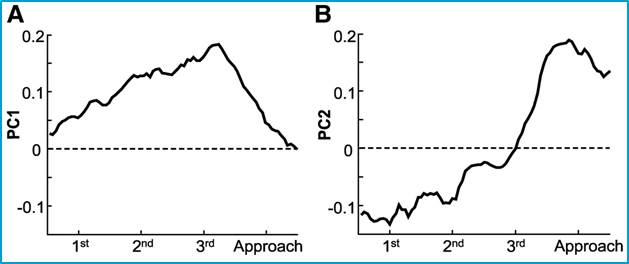
\includegraphics[width=0.5\textwidth]{LyaPca}
%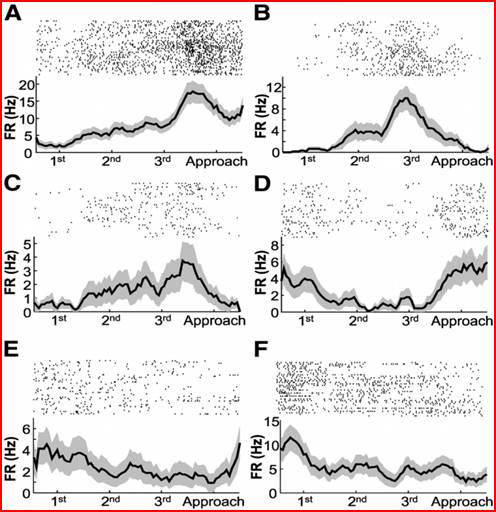
\includegraphics[width=0.5\textwidth]{LyaPcaCon}
%\caption{\footnotesize{\textbf{Left}: The main patterns of firing rate variance in ACC as detected in PCA analysis, A. First eingenvector, B. Second eingvector}, \textbf{Rigth} Examples of progressive firing rate patterns exhibited by ACC neurons. Top: Raster plot; Bottom: Average firing rates across trials. A-C: examples of neurons positively loaded in both PC1 and PC2 (case A) or PC1 only (case B,C). D-F: examples of neurons negatively loaded on PC1. Figure reproduced and modified from (\cite{Lya})}
%\label{fig: LyaPca}
%\end{figure}
From those analysis the authors conclude that the neurons in ACC exhibit an activation on a specific moment of the task, e.g. the lever press moment or the reward (consumption or assumption), without discrimination among different sequences. The neurons codify for the order of the lever press; the position of the lever doesn't play any role in this codification. That means that if one pair of neurons in the ACC codify for the first lever press in the first sequence, it keep to codify for the first lever in the second and in the third sequence block, even when the first lever is placed in another point of the space. In figure (\ref{fig: ACC_assembly}) examples of ensambles found with the cell assemblies algorithm, that show agreement with previous result. We remember that at the end of each sequence block the sensory cues were moved to different levers. 
PCA analysis reveal that DS neurons instead showed two kind of behavior, one characterized by strong variations in association with each lever press followed by an abrupt decline during the reward-approach epoch; another one characterized by a strong variation on the reward approach epoch. With the cell assembly algorithm we find a strong variation during the reward-approach epoch and more interestingly an activation on the lever press that is differentiate not by the order the lever but by the location of the lever, that means a discrimination among different sequences performed by DS ensembles (see \cite{Lya}). In (\cite{LyaN}) is also shown that the capability to discriminate among sequences is much clear looking at pattern of neurons than at single units level. We find this capability very clearly already at pairs level, with the cell-assembly- detection- algorithm, as we show in figure (\ref{fig: DS_Assembly}).
In figure (\ref{fig: DS_Assembly}) we can see in fact that pairs codifying for example for the right lever are almost silent during the pressing of the left or the middle lever. We detect a pattern responding to specific place of the space that is silent in the moments of the task in which this position is not involved.
\begin{figure}
    \centering
    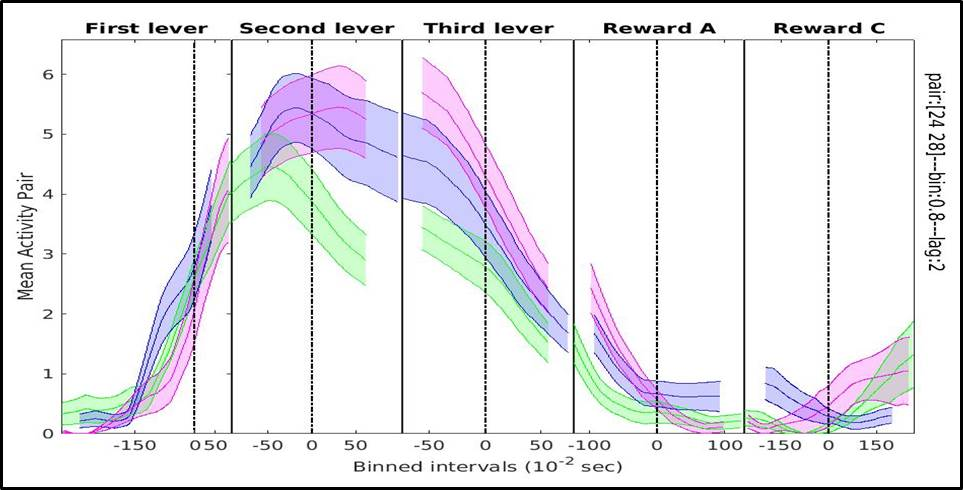
\includegraphics[width=0.44\textwidth]{ACC1}
    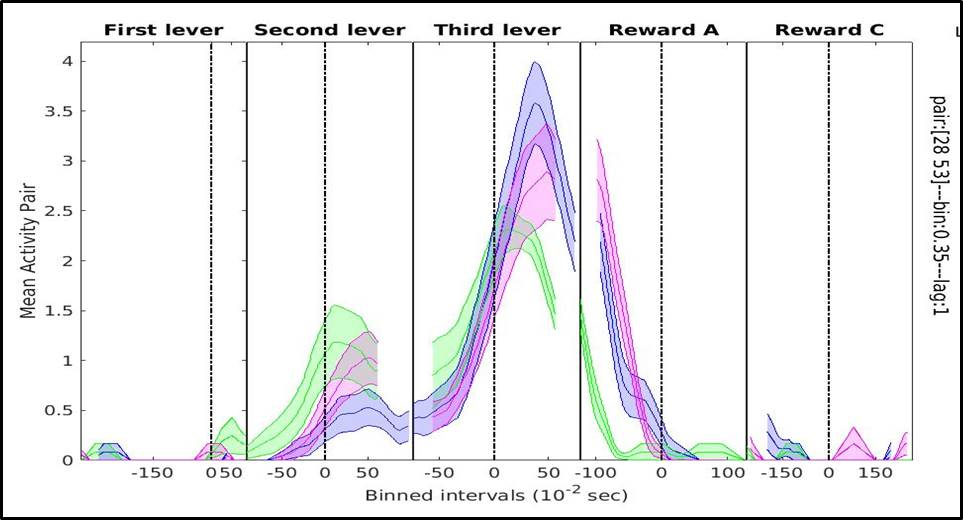
\includegraphics[width=0.415\textwidth]{ACC2}
    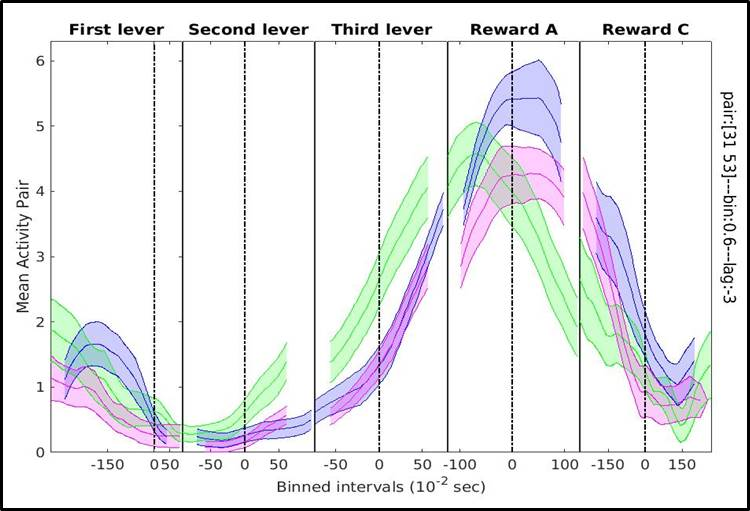
\includegraphics[width=0.44\textwidth]{ACC3}
   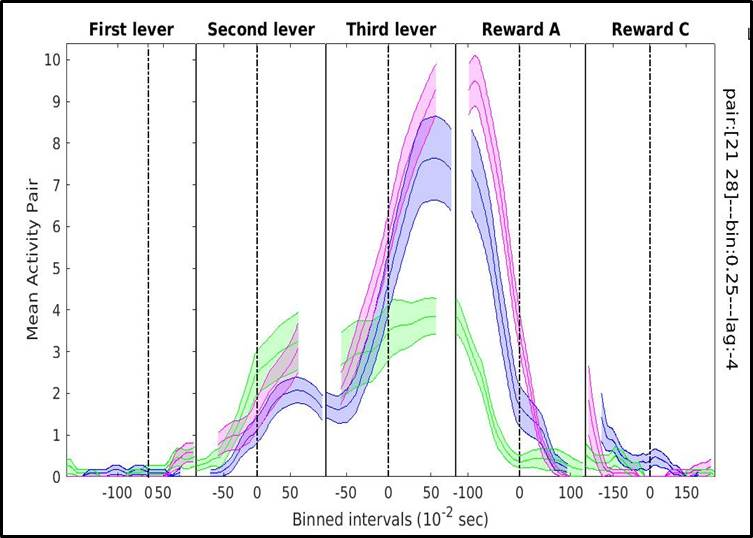
\includegraphics[width=0.415\textwidth]{ACC4}
  \caption{\footnotesize{ACC cell assemblies examples. Different colors stay for different sequences blocks. Ensembles of neurons in PCA respond to a particular moments of the task (lever press, reward) showing any preference of discrimination for the different sequences blocks of the experiment, namely they don't codify for left/right/middle levers.}}
   \label{fig: ACC_assembly}
 \end{figure}
%\begin{figure}
%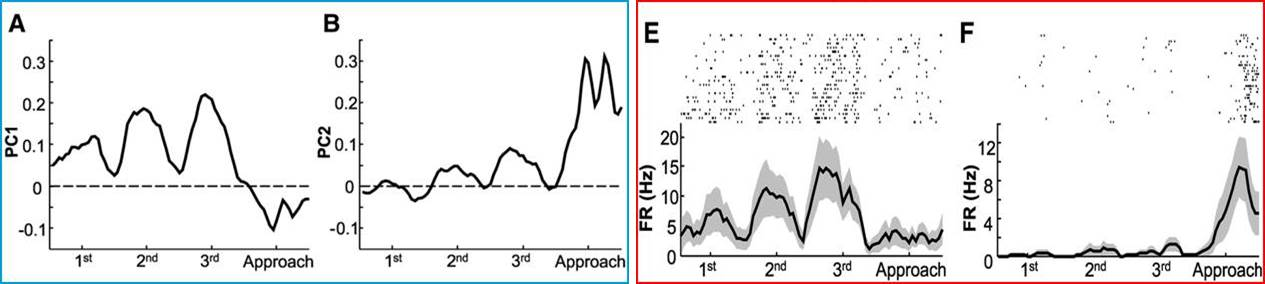
\includegraphics[width=1\textwidth]{LyaDS_PCA}
%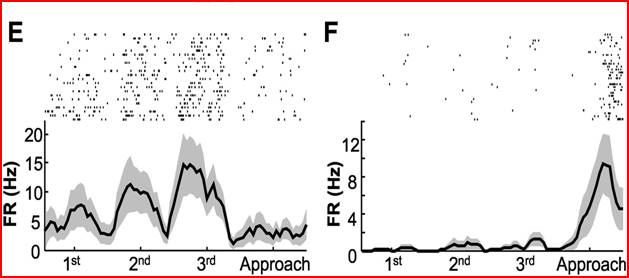
\includegraphics[width=0.5\textwidth]{LyaPcaDSCon}
%\caption{\footnotesize{\textbf{Left}: The main patterns of firing rate variance in DS as detected in PCA analysis, A. First eingenvector, B. Second eingenvector}, \textbf{Rigth}Examples of the progressive firing rate patterns exhibited by DS neurons.Top: Raster plot Bottom: Average Firing rate across all trials
%E. Example of a single neuron strongly loaded on both PC1 and PC2
%F. Example a single neuron strongly loaded on PC2. Figure reproduced and modified by (\cite{Lya})}
%\label{fig: LyaPCADS}
%\end{figure}
\begin{figure}
    \centering
    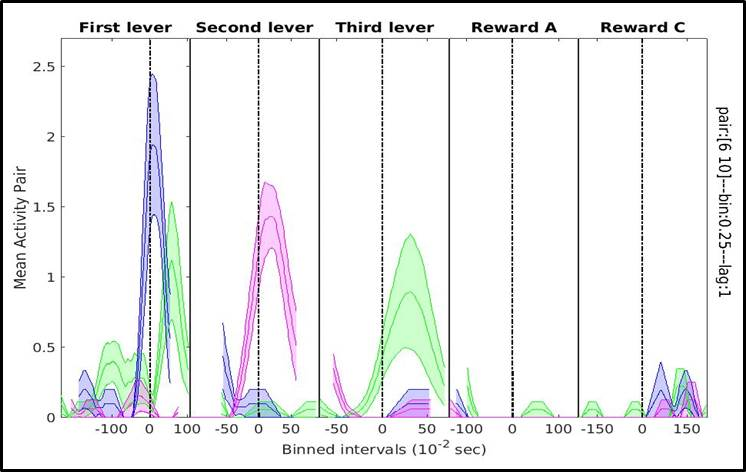
\includegraphics[width=0.45\textwidth]{DS1}
    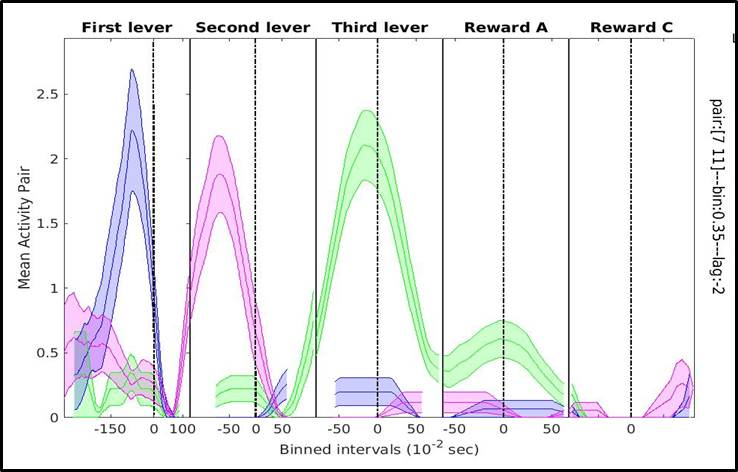
\includegraphics[width=0.445\textwidth]{DS2}
    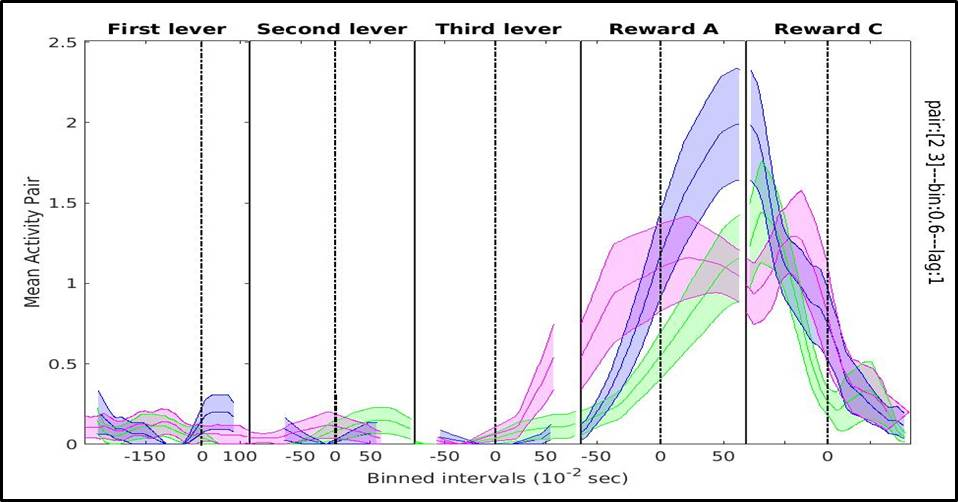
\includegraphics[width=0.45\textwidth]{DS_r1}
    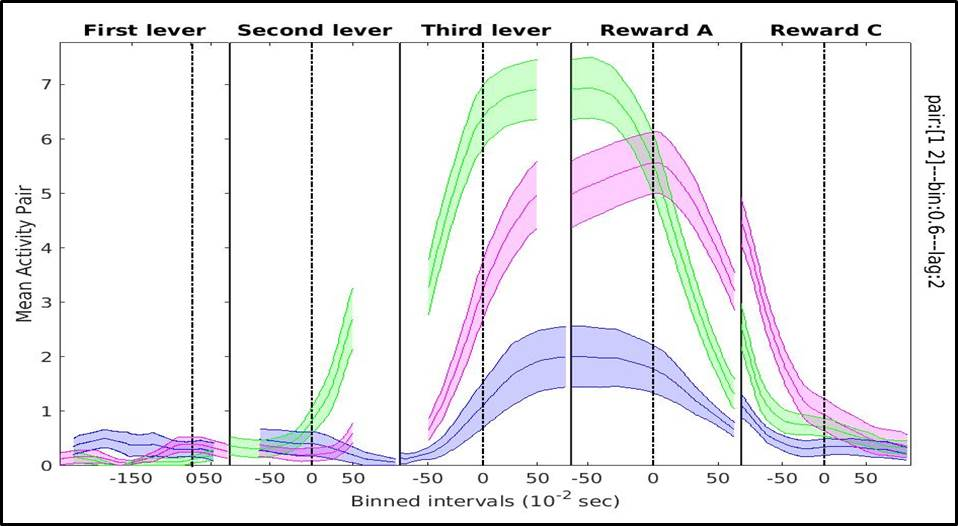
\includegraphics[width=0.445\textwidth]{DS_r2}
    \caption{\footnotesize{Example of ensemble of DS neurons. \textbf{Top}: Example of lever codification by DS neurons, as we can note, looking at the assembly the lever codification/sequences discrimination is more clear and emphasized than in single neuron case. In fact here we can observe a clear activation of the assembly only and univocally on the right level, that had to be pressed as first, second or third level depending to the sequence. \textbf{Bottom}: Codification of DS neurons for the reward.}}
    \label{fig: DS_Assembly}
\end{figure}
\subsection{Inter area communication and information transfer}
\textbf{Second data set. Neurons within VS and VTA recorded in odour discrimination task.}
For multi-site recordings. The distribution of time lags between the activation of units of an
ensemble recorded across different areas can give an insight in the causal interaction
between the two regions in a temporally resolved manner (Figure \ref{fig: pairs_and_single}).
In Figure (\ref{fig: LagBinDistr}) are shown the distribution of activation lags between Ventral Striatum - Ventral Tegmental Area interaction,  and the distribution of the Bin sizes in an odour discrimination task. From the lag distribution we argue that at a temporal resolution of 30-120 ms VS leads VTA activation. Positive lags correspond to VS unit preceding VTA unit activation, negative lags vice versa.
From The bin distribution is interesting to notice a bimodality that remarks a segregetion in time.
\begin{figure}
    \centering
    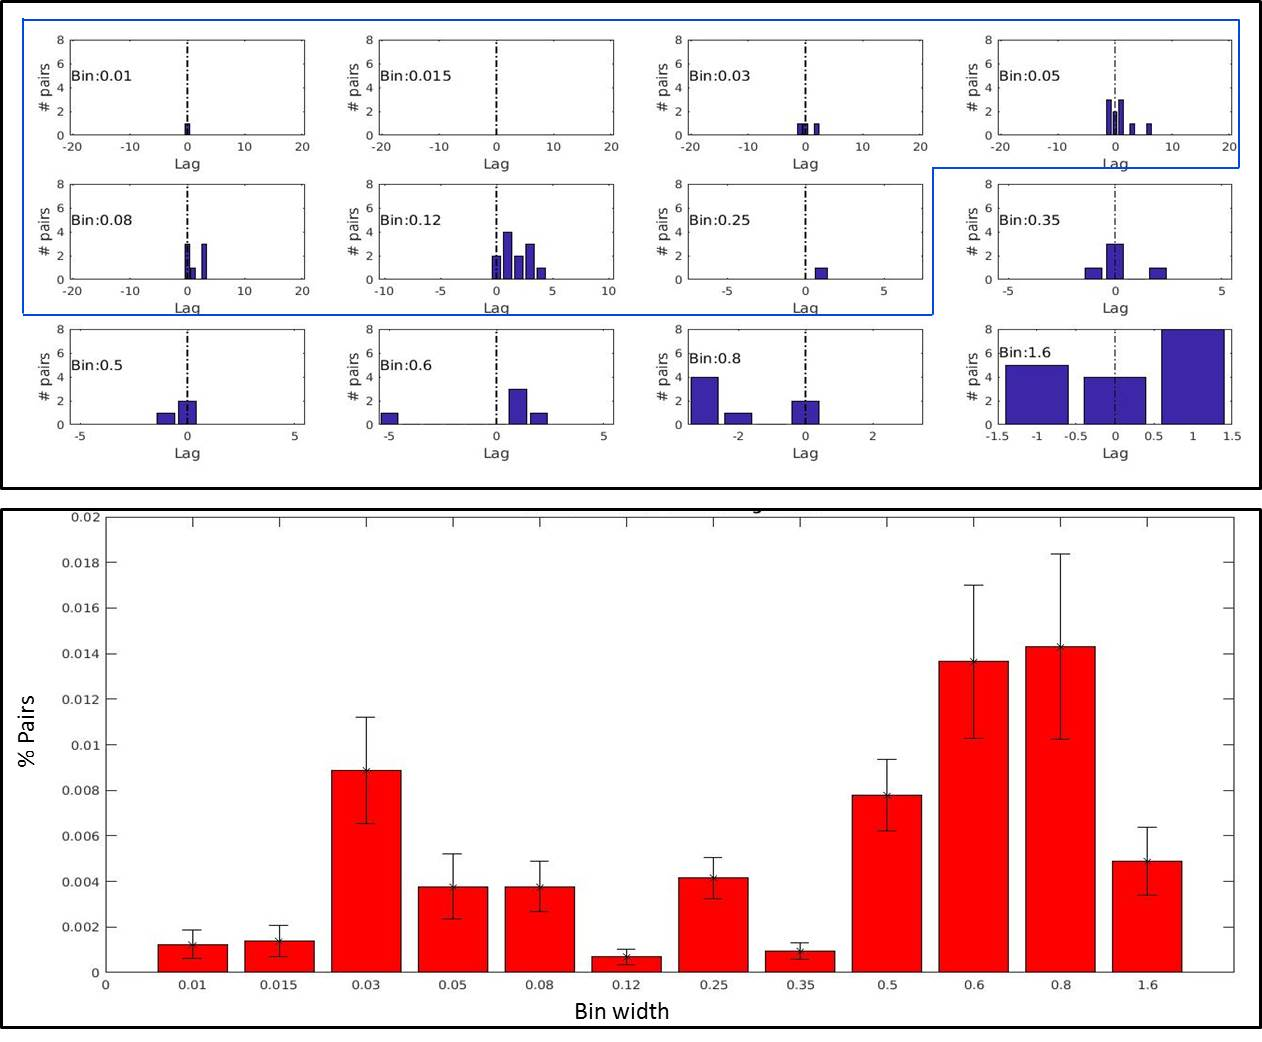
\includegraphics[width=0.9\textwidth]{LagBinDistr}
    %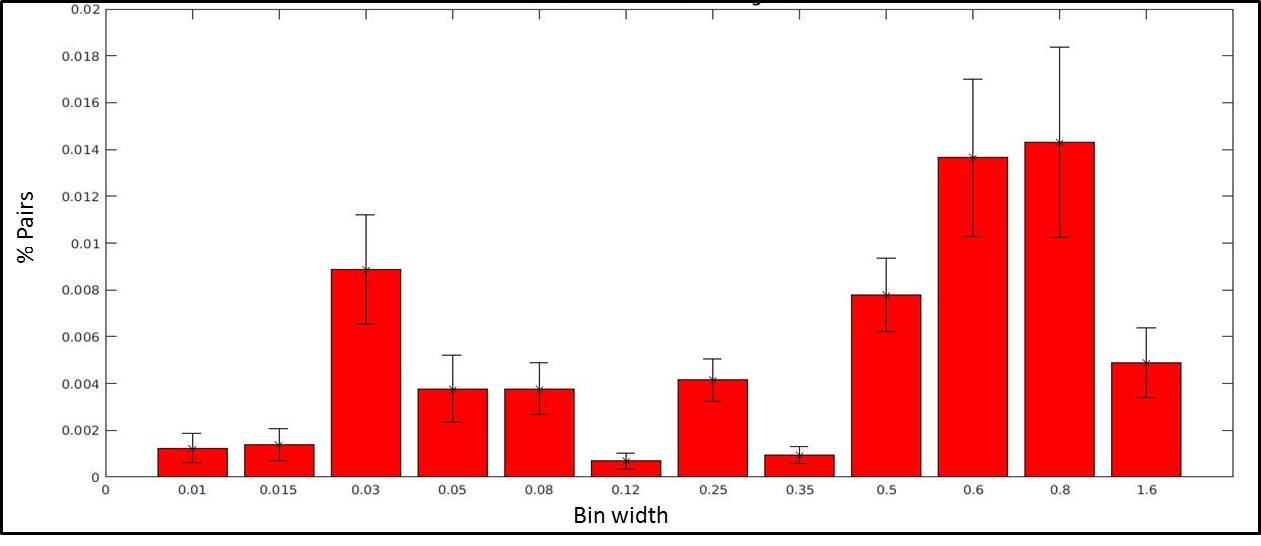
\includegraphics[width=0.9\textwidth]{BinDistr}
    \caption{\footnotesize{\textbf{Top} Dual site VS – VTA recordings during an odour discrimination task in mice. Distribution of activation lags between
(VS,VTA) pairs detected as ensemble with 50 ms binning resolution. Positive lags correspond to VS unit preceding VTA unit activation, negative lags vice versa.\text{Bottom} Distribution of activation bins between (VS,VTA) pairs detected as ensemble. The distribution is bimodal and suggests a time segregation.}}
    \label{fig: LagBinDistr}
\end{figure}
A segregation in time is highlighted both from the lag distribution and the bin width distribution (fig. \ref{fig: LagBinDistr}).
%\begin{figure}
 %   \centering
 %   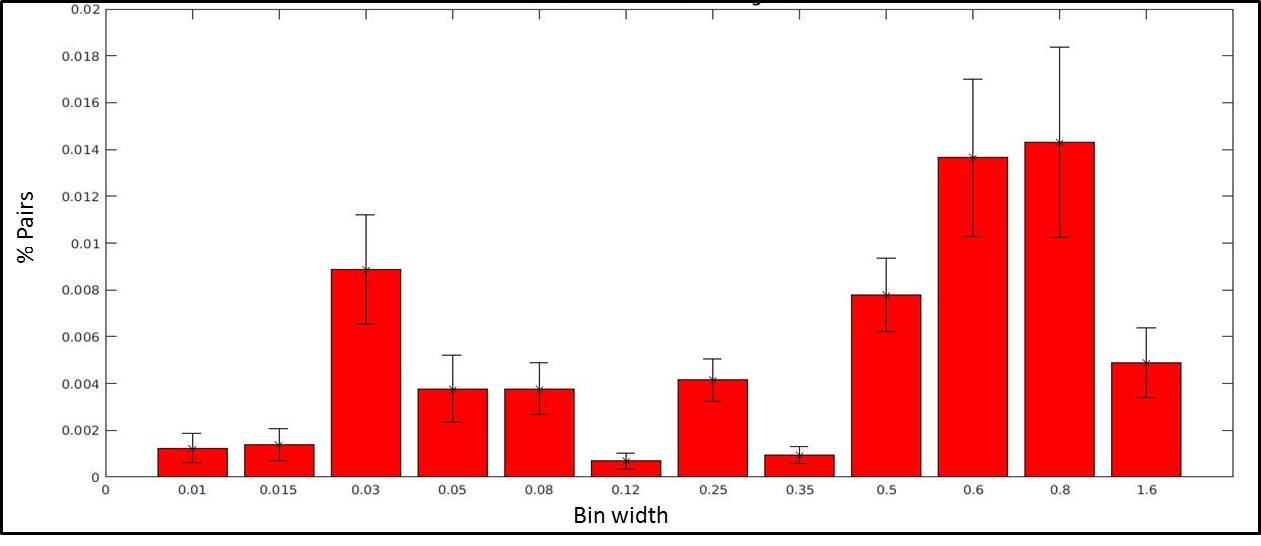
\includegraphics[width=1\textwidth]{BinDistr}
  %  \label{fig: BinDistr}
%\end{figure}
Figure (\ref{fig: AssemblyAct}) shows that the temporal segregation emerged from the bin width analysis divides assemblies in distinct activation profiles.
\begin{figure}
    \centering
    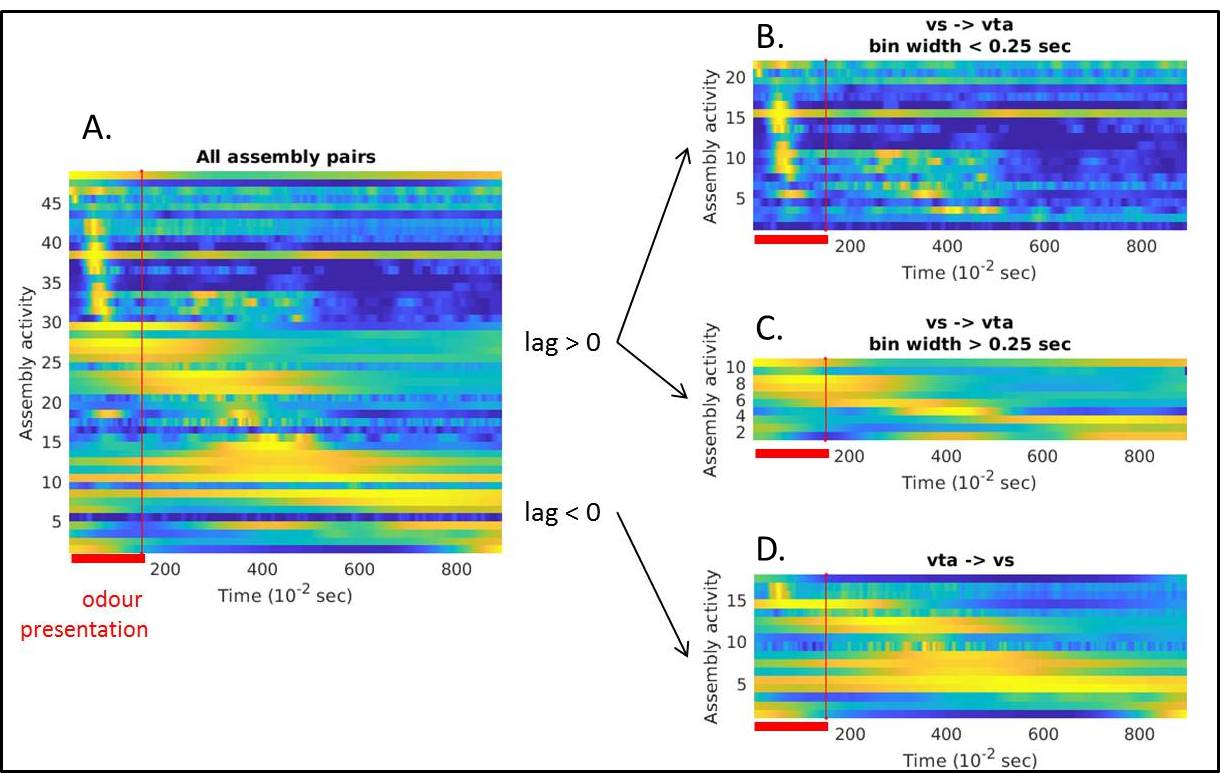
\includegraphics[width=1\textwidth]{AssemblyAct}
    \caption{\footnotesize{The temporal segregation emerged from the bin width analysis divides assemblies in distinct activation profiles. \textbf{A.} Mean activity of all the assemblies pairs shared between DS and VTA. \textbf{B.} Activity of those ensembles with positive lag and bin width $<$ 0.25 sec. \textbf{C.} Activity of those ensembles with positive lag and bin width $>$ 0.25 sec. \textbf{D.} Activity of those ensembles with negative lags}}
    \label{fig: AssemblyAct}
\end{figure}
\begin{figure}
    \centering
    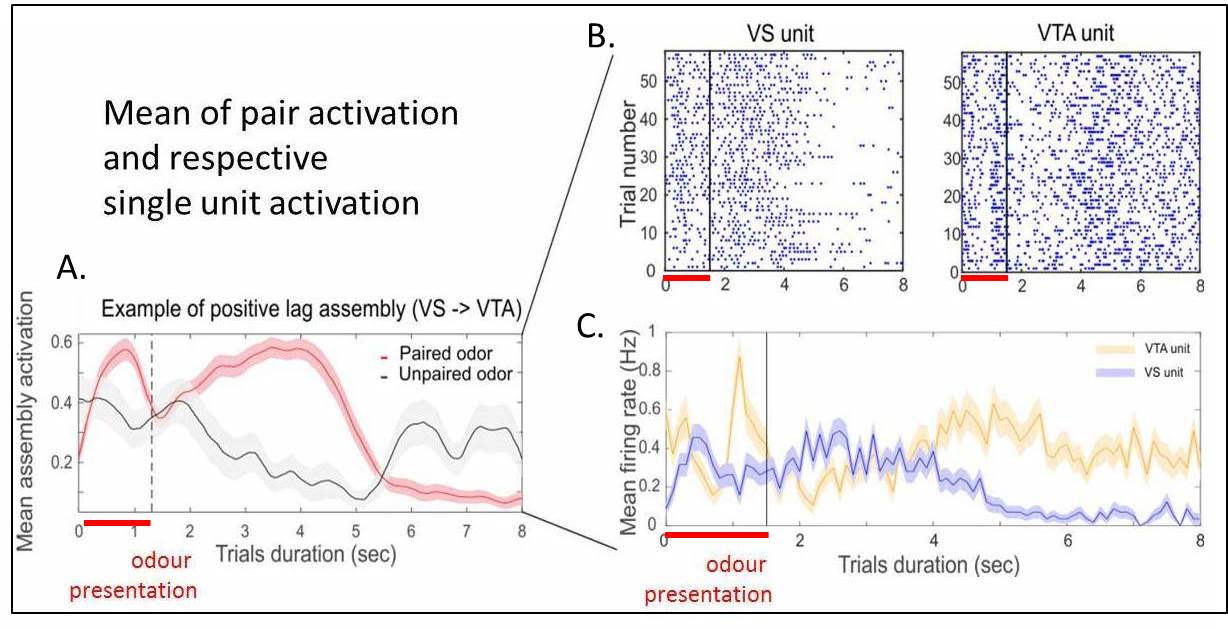
\includegraphics[width=1\textwidth]{pairs_and_single}
    \caption{\footnotesize{\textbf{A.} Example of mean activation of a positive-lag ensemble during trials. The ensemble discriminates between paired and unpaired odour. \textbf{B ,C.} raster plot and mean firing rate of the two units composing the ensemble depicted on A. Single unit activations confirm the temporal relation highlighted by the ensemble analysis. Data provided by Wolfgang Kelsh (project C04).}}
    \label{fig: pairs_and_single}
\end{figure}
We focus on those pairs with positive directionality. In figure(\ref{fig: pairs_and_single}) is shown an example of mean activation of positive lag ensemble during the trials. The ensemble is able to discriminate between rewarded and not rewarded odor.
The single unit activity on the left-bottom side of the figure({\ref{fig: pairs_and_single}}) confirm the temporal relationship highlighted by the ensemble analysis.
\subsection{Future steps}
We are interested principally in two characterization of the assembly. The first characterization, that we partially already shown, is the coding by the ensemble in different task moments.
The second characterization is related to the identity of the ensembles. Recent studies show the presence of neuron-type-specific signals in different task moments both in Ventral Striatum and in Ventral Tegmental Area (\cite{Atallah}, \cite{Cohen}). Looking at types of neurons involved in the ensemble, we are able to characterize ensemble types, and to see whether there exist ensemble-type-specific information.

\section{Conclusion}
One of the peculiarity of neuronal systems is the presence of different time scales in the neural response to a specific task. This beauty is unfortunately not easy to detect in the ensemble analysis context: the major part of ensemble methods in fact are able to find activation patterns only at one of the several time scales present, with a consequent big information loss.
Another factor that plague data analysis in neuroscience is the presence of non-stationarity artefacts in experimental data.
The cell assembly algorithm allow us to detect specific activation patterns in presence of multiple time scales and in non-stationarity conditions.
Its application on real data not only confirm that huge amount of information is carried by patterns of neurons, but also reveals interesting time segregation in pairs detected in VS and VTA in odour discrimination that divide the assemblies in different activation profiles. The time segregation, possible only because the algorithm is able to capture different time scales of the neural network, come to be a crucial point in the information carried by the ensembles.
\newpage

\printbibliography
%\renewcommand{\refname}{\spacedlowsmallcaps{Brief list of principle references}} % For modifying the bibliography heading

%\bibliographystyle{unsrt}


%\bibliography{sample.bib} % The file containing the bibliography
%\begin{thebibliography}{triangle}

%\bibitem[Russo, Durstewitz, 2017]{RussoDurstewitz}
%E. Russo, D. Durstewitz: 
%\newblock{Cell assemblies at multiple time scales }
%\newblock{\textit{2nd ed. Chapman \& Hall,London}. (1989) }



%\end{thebibliography}


\end{document}



